\clearpage
\chapter{Optimal Deployment of Energy Harvesters with Anti-correlated Energy Generation Profiles at Base Stations\label{Chapter_3}}
\settablecounter{4}{1}

Chapter \ref{Chapter_3} will extend the previous system model to a multi-cell cellular network.
There are now several BSs distributed in an area and some of them are connected by distribution lines to share the renewable energy among them. The problem investigated in this chapter is how renewable energy harvesters (e.g., a PV cell or a small wind turbine) with anti-correlated energy generation profiles should be deployed to every BS so that the renewable energy can be shared most efficiently in the multi-cell cellular network. Two PV cells that have significantly different orientation angles, such as east-oriented and west-oriented PV cells, are an example for energy harvesters with anti-correlated energy generation profiles. 







\section{Background: Different Power Sharing Methods}
The amount of harvested power as well as the power consumption of the BSs vary over time and space resulting in power surpluses or power deficits at the BSs. To avoid wasting precious harvested power, power can be transmitted from surplus BSs to deficit BSs via distribution lines. Other options for power sharing are wireless power transfer, traffic offloading, smart grid/ main grid trading and batteries. These options are discussed separately and are compared with power sharing via distribution lines in the following sections.

\subsection{Wireless Power Transfer}
Power can be shared through wireless power transfer. Nonetheless, this is limited to very short distances due to the high power losses associated with long wireless power transmission \cite{7437420}.
\subsection{Traffic Offloading}
The authors in \cite{7273976} proposed to offload UEs at the cell edge of BSs with power deficit to neighboring BSs with power surplus. The authors in \cite{WildemeerschMatthias2013CSCN,Pei-ShanYu2016TOiH} proposed to offload UEs from tiers with power deficit to tiers with power surplus, e.g., between macro BSs and small BSs, in a heterogeneous cellular network. The authors in \cite{JingjinWu2015EBST,Huang2017,MinWookKang2017AEES} proposed to offload UEs from BSs with power deficit to BSs with power surplus by switching BSs with power deficit into a sleep mode. Nonetheless, traffic offloading causes a deterioration in the signal-to-interference-plus-noise ratio (SINR) of the offloaded UEs, whereas power sharing via distribution lines does not affect the SINR.
\subsection{Smart Grid/ Main Grid Trading}
The authors in \cite{7779131, 7841800} proposed to sell and buy power from the grid and use the grid to conduct virtual power transfer in addition to power sharing via distribution lines. Power sharing via distribution lines requires high capital expenditure for deploying physical distribution lines, whereas grid trading implies operational expenditure in the form of a price that has to be paid to the grid operator. To evaluate if the initial investment for deploying physical distribution lines is justified in the long-term or each BS should rather sell and buy its power from the grid, the local price structure has to be evaluated. BSs can buy power from the grid at a price $p_b$ and sell it to the grid at a price $p_s$ (feed-in tariff), where the grid operator typically requires that $p_b > p_s$ \cite{JieXu2016CETi}. The difference in price, denoted by $\Delta_p$, is as follows: $\Delta_p=p_b-p_s$ \cite{JieXu2015Cgcn}. 
If $\Delta_p$ is great, it is more cost-efficient to share power via distribution lines. If  $\Delta_p$ is small, it is more cost-efficient to sell and buy power from the grid. Even if  $\Delta_p$ is small, cellular network operators may prefer to rely on their own local power sharing infrastructure to avoid reliance on the grid and to avoid the risk of future power price changes beyond their control. In general, power sharing via distribution lines is usually cost-efficient in dense cellular networks with small to medium inter-site distances, where the power losses in the distribution lines are low, expensive step-up and step-down transformers are not needed, and direct current (DC) to alternating current (AC) conversion losses are negligible or DC distribution lines are deployed between DC energy harvesters, such as PV cells.  
In contrast, sparse cellular networks with long inter-site distances are not suitable for power sharing via distribution lines due to the high power losses in the distribution lines, the high capital expenditures, and the right-of-way clearances needed for the transmission corridors. In the latter case, power will be more likely bought and sold to the grid.
\subsection{Batteries}
Since batteries are expensive and have a short lifetime (3 - 9 years), battery replacements significantly contribute to the system lifetime cost \cite{CROSSLAND201530}. Employing both, distribution lines for power sharing and batteries to balance the mismatch between the power generation and consumption at the BSs, would greatly increase the capital expenditures. Hence, only distribution lines are considered in the system model of Chapter \ref{Chapter_3} to reduce the capital expenditures. Nonetheless, if batteries are deployed as well, efficient power sharing algorithm can reduce the required battery capacities, as seen in \cite{BingyuXu2017EPCi}.






\section{Literature Review: Benefits of Anti-correlated Energy Generation}


BSs powered by renewable energy face the problem of temporal variations in the energy supply. These variations have to be managed properly to make efficient use of the harvested renewable energy. Energy harvesters with anti-correlated energy generation can mitigate the temporal variations in the energy supply. Thus, the energy deficit in one profile can be compensated by an energy surplus of another profile. For instance, 80\% of energy was saved in \cite{6874568} between a pair of energy-sharing BSs with anti-correlated sinusoidal energy profiles. 


Instead of relying on only one energy source with one only characteristic energy generation profile, it is recommended to rely on a mix of different energy sources with anti-correlated energy generation profiles. 
The benefits of relying on a mix of different energy sources have been comprehensively studied in smart grids and conventional power grids \cite{ValdesLucas20161032, Li20052237, auf,JieXu2015CMSG}. Relying on a mix of different renewable energy sources to power cellular networks has been mainly studied in literature by combining wind energy and solar energy \cite{residential, white_energy}. The anti-correlation between solar and wind energy generation profiles is justified on a daily timescale by the fact that high pressure (low pressure) areas tend to be sunny (cloudy) with low (high) surface wind, and on a seasonal timescale by the fact that solar (wind) energy is higher in summer (winter) than in winter (summer) for many locations \cite{white_energy}. 


It is especially promising to connect nearby BSs with power distribution lines \cite{8491374,my_con3,7143338} and to deploy energy harvesters with anti-correlated energy generation profiles at nearby BSs that are connected by power distribution lines. As a result, power can be transmitted from surplus BSs to deficit BSs via short distribution lines and the distance-dependent power losses in the distribution lines are small. Most papers in the literature do not consider the distance-dependent power loss in the distribution lines. For example, \cite{XueqingHuang2017SGEM} introduced an energy hub for power sharing in cellular networks but assumed that the resistive power loss in the distribution lines is independent of the power propagation distance.

On the one hand, the greater the distance between two PV cells, the more anti-correlated are their energy generation profiles and the more power can be transmitted from the surplus BS to the deficit BS \cite{HoffThomasE.2012MPfo,leeds}. On the other hand, the greater the distance between two PV cells, the more power is lost in the distribution line.


\section{Proof of Concept}


To demonstrate the concept of energy harvesters with anti-correlated energy generation profiles, a southeast-orientated PV cell 
(energy harvester type 0) and a southwest-orientated PV cell (energy harvester type 1) in Greenwich (London, UK) in June are used as an example. Southeast-, and southwest-orientated PV cells have an orientation angle of $-45^{\mathrm{o}}$, and $45^{\mathrm{o}}$ with respect to the southern direction, respectively (cf. Figure \ref{angle}). While energy harvester type 0 has a high power generation during time step 1 (potential surplus), energy harvester type 1 suffers from a low power generation (potential deficit), as seen in Figure \ref{example}. Vice versa in time step 2, while energy harvester type 0 has a low power generation (potential deficit), energy harvester type 1 has a high power generation (potential surplus). Each BS is deployed with one of the two energy harvester types and all BSs have the same constant energy consumption profile for simplicity in this example, as seen in Figure \ref{example}. To make efficient use of the renewable power, power should be transmitted via distribution lines from BSs equipped with energy harvester type 0 to BSs equipped with energy harvester type 1 in time step 1. Vice versa in time step 2, power should be transmitted via distribution lines from BSs equipped with energy harvester type 1 to BSs equipped with energy harvester type 0.




\begin{figure}[H]
\centering
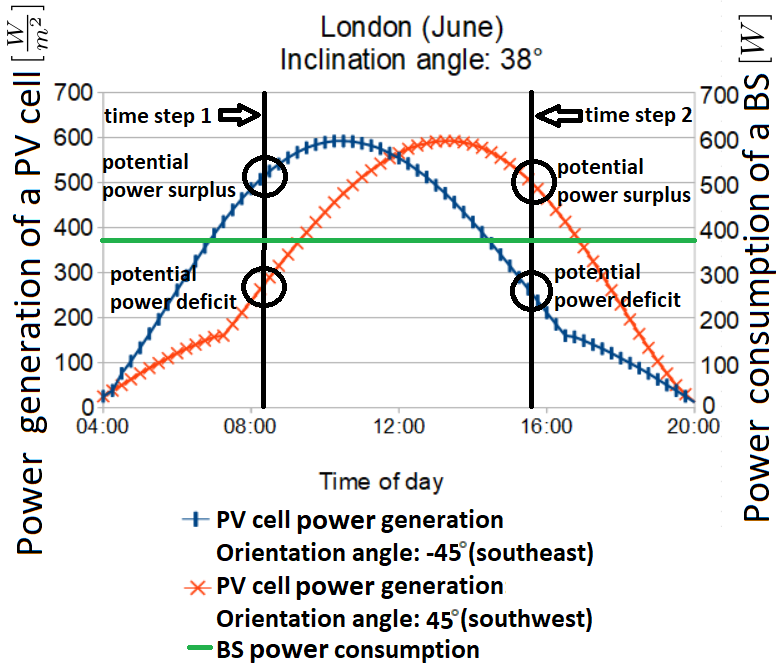
\includegraphics[width=0.9\columnwidth]{pictures/3}
\caption[Demonstration of the concept of energy harvesters with anti-correlated energy generation profiles]{A southeast-orientated PV cell and a southwest-orientated PV cell in Greenwich (London, UK) in June are used to demonstrate the concept of energy harvesters with anti-correlated energy generation profiles. The historical average time series data of the PV cells were derived from PVGIS \cite{PVGIS}.\label{example}}
\end{figure}


\section{Contributions of Chapter \ref{Chapter_3}}
The contributions of Chapter \ref{Chapter_3} are summarized as follows:

\begin{itemize}
\item  Developing an optimization algorithm that can be run once during the cellular network planning to determine what type of energy harvesters should be deployed to every BS in a cellular network. There are two different types of energy harvesters available for deployment which have anti-correlated energy generation profiles.
\item Taking into account the topology of the cellular network as well as the distance-dependent power loss in the distribution lines during the optimization.
\item Developing an optimization objective that maximizes the power that can be transmitted from surplus BSs to deficit BSs in the cellular network.
\item Comparing the proposed optimization algorithm with randomly deploying anti-correlated energy harvesters to the BSs. The effects of different numbers of BSs, different distribution line existence probabilities, different distribution line power loss coefficients, and different power surplus values are investigated. 
\end{itemize}

\section[System Model 3 - Deployment of Anti-correlated Energy Harvesters]{System Model 3 - Deployment of Anti-correlated Energy Harvesters to Every BS in a Cellular Network\label{system_model_3} }


There are $B \in \mathbb{N}$ uniformly distributed BSs in a square area of $l^2$ square meters, $l \in \mathbb{N}$, which are denoted by $BS_i$, $i\in\{1,...,B\}$ (cf. Figure \ref{fig:1}). The parameter $c_i\in\{0,1\}$ denotes if $BS_i$ is equipped with the energy harvesting device type 0 or the energy harvesting device type 1, e.g., either with a solar cell or a wind turbine. A $BS_i$ with energy harvesting device type 0, i.e., $c_i=0$, belongs to cluster 0 and is depicted with a black node in Figure \ref{fig:2}. A $BS_i$ with energy harvesting device type 1, i.e., $c_i=1$, belongs to cluster 1 and is depicted with a red node in Figure \ref{fig:2}. 


The BS clustering optimization algorithm will be run once during the cellular network planning to determine for every BS its cluster and the corresponding energy harvesting device type.

\subsection{Power Surplus/Deficit Values}


The difference between the power generation and consumption of $BS_i$ is denoted by the power surplus/deficit value $p_i^t [W]$ in watts for time step $t\in\{1,2\}$. A surplus in power, and a deficit in power at $BS_i$ are indicated by a positive value $p_i^t$, and a negative value $p_i^t$, respectively. The power surplus/deficit values of BSs in the same cluster at a given time step are similar because they are equipped with the same energy harvesting device type and have a similar BS load. As a result, all BSs in the same cluster are assumed to have the same power surplus/deficit value at a given time step.



The energy generation profile of BSs in cluster 0 is anti-correlated to the energy generation profile of BSs in cluster 1. In other words, BSs of cluster 0, and cluster 1 have a power surplus of $b_0\in \mathbb{R^+}$, and a power deficit of $b_1\in \mathbb{R^-}$ in time step 1, respectively. Vice versa in time step 2, BSs of cluster 0, and cluster 1 have a power deficit of $b_1$, and a power surplus of $b_0$, respectively. The power surplus/deficit values $p^t_i$\footnote{It is assumed that every BS has a similar total daily energy consumption. Therefore, the energy harvesting device types should have similar capacities. The capacity of an energy harvesting device should not be oversized or undersized for powering one BS, that means it can be assumed that every BS will experience power surpluses and power deficits throughout the day.  
The time during a day where energy harvesting device 0 produces more power than the energy harvesting device 1 is represented by time step 1, whereas the time during a day where energy harvesting device 1 produces more power than the energy harvesting device 0 is represented by time step 2. Hence, it is justified to use only two time steps $t\in\{1,2\}$ in the system model 3 to represent a 24-hour day. Because the optimization is done only once in a BS's lifetime, $p^t_i$ represents the average daily power surplus/deficit value at the BS throughout the lifetime of the BS. Thus, it can be assumed that throughout the lifetimes of the BSs, the power surplus/deficit values at the BSs in the same cluster at a given time step are the same because they are equipped with the same energy harvesting device type and have a similar BS load. 
Because the energy harvesting device types have similar capacities, it can be assumed that $p^1_0=p^2_1=b_0$ and $p^1_1=p^2_0=b_1$.} are summarized as follows:


\begin{equation}\label{p_values}
\begin{aligned}
&p^t_i=\begin{cases} 
			b_0& \quad  c_i=0 \text{ and }t=1 \\
		b_1 &\quad  c_i=1 \text{ and }t=1\\
			b_1& \quad  c_i=0 \text{ and }t=2 \\
		b_0 &\quad  c_i=1 \text{ and }t=2.
   \end{cases}
	\end{aligned}
\end{equation}



\begin{figure}[H]
\centering 
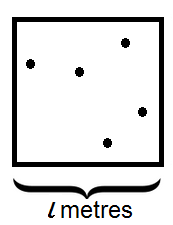
\includegraphics[width=0.3\columnwidth]{pictures/square4}
\caption[Illustration of the considered cellular network]{Illustration of the considered cellular network with $B=5$ BSs uniformly distributed in a square area of $l^2$ square meters. \label{fig:1}}
\end{figure}


\begin{figure}[H]
\centering 
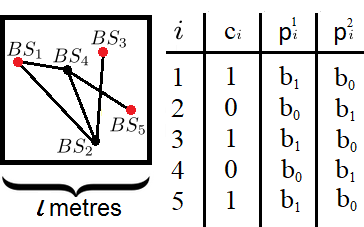
\includegraphics[width=0.6\columnwidth]{pictures/square6}
\caption[The graph representation of the cellular network]{The graph representation of the cellular network with example BS cluster allocation values $c_i$, surplus/deficit power values $p_i^1$ in time step 1 and surplus/deficit power values $p_i^2$ in time step 2 given for the BSs.\label{fig:2}\label{area}}
\end{figure}

\subsection{Distance-dependent Power Loss in the Distribution Lines}
The normalized Euclidean distance $d\big((i,j)\big)$ between $BS_i$ and $BS_j$ with respect to $l$ meters is as follows:


\begin{equation}\label{equ_y}
d\big((i,j)\big)=\frac{||BS_i-BS_j||}{l},
\end{equation}




\noindent
where $||BS_i-BS_j||[\mathrm{m}]$ in meters is the Euclidean distance between $BS_i$ and $BS_j$, and $l[m]$ in meters is the side length of the square in Figure \ref{fig:2}.

Power can be transmitted from a surplus BS in one cluster to a deficit BS in the other cluster at each time step if the two BSs are connected by a distribution line. The power flow in the distribution line is subject to power loss due to resistive heating. The power loss $P_{\mathrm{loss}}\big((i,j)\big)[\mathrm{W}]$ in watts in the distribution line from $BS_i$ to $BS_j$ can be calculated by Ohm's law and the formula for the distribution line resistance \cite{Resis} as follows:


\begin{equation}\label{loss}
P_{\mathrm{loss}}\big((i,j)\big)=I_{\mathrm{ele}}^2\cdot \rho\cdot  \frac{l \cdot d\big((i,j)\big)}{A_{\mathrm{c}}}=I_{\mathrm{ele}}^2\cdot C \cdot d\big((i,j)\big),
\end{equation}




\noindent
where $I_{\mathrm{ele}}[\mathrm{A}]$ in amperes is the electric current traveling through the distribution line, $\rho[\mathrm{\Omega m}]$ in ohm-meters is the resistivity of the distribution line, $l[\mathrm{m}]$ in meters is the side length of the square in Figure \ref{fig:2}, $d\big((i,j)\big)$ is defined in (\ref{equ_y}), $A_{\mathrm{c}}[\mathrm{m^2}]$ in square meters is the cross-sectional area of the distribution line, and $C[\mathrm{\Omega}]$ in ohms is the power loss coefficient
per $l$ meters of distribution line, i.e., $C=\frac{\rho\cdot l}{A_c}$.


\subsection{Topology of the Cellular Network}
The topology of the cellular network is represented by a graph (cf. Figure \ref{fig:2}), where $V$ is the set of vertices which denotes the BSs, and $E$ is the set of directed edges which denotes the distribution lines as follows:



\begin{equation}
\begin{aligned}\label{V_and_E}
V=&\{1,2,...,B\},\\
E=&\{(i,j),(j,i)|i\in V, j\in V, \text{$BS_i$ and $BS_j$ are } \\
& \text{connected by a distribution line}\},
\end{aligned}
\end{equation}



\noindent
where $(i,j)$ denotes the directed edge from $BS_i$ to $BS_j$.


The power flow on the edge $(i,j)$ is denoted by $f^t\big((i,j)\big)$ in time step $t\in\{1,2\}$.

All power values are normalized with respect to the constant value of $\max\{b_0,|b_1|\}$ as follows:


\begin{equation}\label{normal}
\begin{aligned}
\hat{f}^t\big((i,j)\big)&=  \frac{f^t\big((i,j)\big)}{\max\{b_0,|b_1|\}}\\
 \hat{b}_0&=\frac{b_0}{\max\{b_0,|b_1|\}}\\
 \hat{b}_1&=\frac{b_1}{\max\{b_0,|b_1|\}.}
\end{aligned} 
\end{equation}

The power values $\hat{f}^t\big((i,j)\big)$, $\hat{b}_0$, $\hat{b}_1$ are the normalized power values of $f^t\big((i,j)\big)$, $b_0$, $b_1$, respectively.


\subsection{Justification of Assumptions}

The following two assumptions in the system model 3 are justified in this section.
\begin{itemize}
\item  Assumption 1: The power flow is equivalent to the second power of the electric current flow in the distribution line.

The electric power $P$ in the distribution line can be calculated as follows:



\begin{equation}\label{Easy}
P=V_{\mathrm{ele}}\cdot I_{\mathrm{ele}},
\end{equation}

\noindent
where $V_{\mathrm{ele}}$ is the electric potential, and $I_{\mathrm{ele}}$ is the electric current. The power loss $P_{\mathrm{loss}}\big((i,j)\big)$ in the distribution line is caused by the electric current and not the electric potential of the power, as seen in (\ref{loss}). Nonetheless, it is outside of the scope of this thesis to model the relationship between the power flow and the electric current flow in the distribution line. Hence, it is assumed for simplicity and in accordance with (\ref{Easy}) that if the power increases/decreases in the distribution line, the electric current and the electric potential increase/decrease equally. In other words, a power flow in the distribution line of $x$ watts is equivalent to a flow of $I_{\mathrm{ele}} = \sqrt{x}$ amperes and $V_{\mathrm{ele}} = \sqrt{x}$ voltages in the system model 3. Hence, the parameter $f^t\big((i,j)\big)[W/A^2]$ can be interpreted as the power flow on the edge $(i,j)$ in watts or the second power of the current flow $I_{\mathrm{ele}}^2$ on the edge $(i,j)$ in square amperes. 
\item Assumption 2: $C\in\big[0,\frac{1}{\sqrt{2}}\big]$.

The maximum normalized distance $d\big((i,j)\big)$ in a square is $\sqrt{2}$. If $C$ were greater than $\frac{1}{\sqrt{2}}$, then $C \cdot d\big((i,j)\big)$ could be greater than $1$. That would imply that more power is lost in the distribution line than was sent through the distribution line. 

\end{itemize}








\section{Mixed-Integer Linear Programming Problem\label{MILPP_pres}}

The objective is to find the optimal BS cluster allocation values $c_n$ for all $BS_n, n \in V$, i.e., deploying either an energy harvesting device type 0 or an energy
harvesting device type 1 at every BS, so that the renewable power in the cellular network can be used most efficiently. $c_n$, $\hat{f}^1\big((i,j)\big)$, and $\hat{f}^2\big((i,j)\big)$ are the parameters to be determined for all $n\in V$ and $(i,j)\in E$. Because the parameters $c_n$ are integers, whereas the power flow values $\hat{f}^t\big((i,j)\big)$ are real numbers, a mixed-integer linear programming solver is needed for this problem. 


The optimization objective is to maximize the total normalized renewable power $M$ received at the deficit BSs during the two time steps as follows:
 


\begin{equation}\label{objective_function}
\begin{aligned}
M=\max_{\substack{c_n,\enskip \hat{f}^1((i,j)), \enskip \hat{f}^2((i,j))\\ \forall n\in V, \enskip \forall(i,j)\in E}} \Big\{&\underbrace{\sum_{(i,j)\in E }\hat{f}^{1}\big((i,j)\big)\big(1-C \cdot d\big((i,j)\big)\big)}_{\text{\normalsize{time step 1}}}\\
+&\underbrace{\sum_{(i,j)\in E }\hat{f}^{2}\big((i,j)\big)\big(1-C \cdot d\big((i,j)\big)\big)}_{\text{\normalsize{time step 2}}}\Big\}\hphantom{safljlllflasd}
\end{aligned}
\end{equation}






\noindent
subject to\\




\noindent
Lower bounds and upper bounds for the parameters to be determined:



\begin{equation}\label{ineq1}
\begin{aligned}
&0 \leq c_n \leq 1,  \quad c_n \in \mathbb{Z}, \quad \forall n\in V\\
 &{\left.0 \leq \hat{f}^1\big((i,j)\big) \leq 1 \quad \forall (i,j)\in E \quad \quad \right\rbrace}\enskip\text{time step 1}\\
 &{\left.0 \leq \hat{f}^2\big((i,j)\big) \leq 1 \quad \forall (i,j)\in E \quad \quad \right\rbrace}\enskip\text{time step 2}
\end{aligned}
\end{equation}




\noindent
Power flow only on edges from surplus BSs to deficit BSs:



\begin{equation}\label{ineq2}
\begin{aligned}
&{\left.\begin{aligned}
&\hat{f}^1\big((i,j)\big) + c_i \leq 1  \quad \forall (i,j)\in E\\
&\hat{f}^1\big((i,j)\big) - c_j \leq 0 \quad \forall (i,j)\in E
\end{aligned} \quad \quad \right\rbrace}\enskip\text{time step 1}\\
&{\left.\begin{aligned}
&\hat{f}^2\big((i,j)\big) + c_j \leq 1  \quad \forall (i,j)\in E\\
&\hat{f}^2\big((i,j)\big) - c_i \leq 0 \quad \forall (i,j)\in E
\end{aligned} \quad \quad \right\rbrace}\enskip\text{time step 2}
\end{aligned}
\end{equation}




\noindent
Power flow out of the surplus BSs:



\begin{equation}\label{ineq3}
\begin{aligned}
 &{\left.\sum_{\substack{(i,j) \in E\\ j\in V}} \hat{f}^1\big((i,j)\big)\leq \hat{b}_0\quad \forall i\in V \quad \quad \right\rbrace}\enskip\text{time step 1}\\
 &{\left.\sum_{\substack{(i,j) \in E\\ j\in V}} \hat{f}^2\big((i,j)\big)\leq \hat{b}_0\quad \forall i\in V \quad \quad \right\rbrace}\enskip\text{time step 2}
\end{aligned}
\end{equation}





\noindent
Power flow into the deficit BSs:



\begin{equation}\label{ineq4}
\begin{aligned}
 &\underbrace{{\sum_{\substack{ (i,j) \in E\\i\in V}} \hat{f}^1\big((i,j)\big)\big(1-C \cdot d\big((i,j)\big)\big)\leq |\hat{b}_1|\quad \forall j\in V }}_{\text{\normalsize{time step 1}}}\\
 &\underbrace{{\sum_{\substack{ (i,j) \in E\\i\in V}} \hat{f}^2\big((i,j)\big)\big(1-C \cdot d\big((i,j)\big)\big)\leq |\hat{b}_1|\quad \forall j\in V }}_{\text{\normalsize{time step 2}}}
\end{aligned}
\end{equation}





The optimization objective (\ref{objective_function}) adds the normalized power flows on all edges and subtracts the normalized power losses (cf. (\ref{loss})) on all edges.


 The inequalities (\ref{ineq1}) represent the lower bounds and the upper bounds for the parameters to be determined, i.e., for the parameters $c_n$, $\hat{f}^1\big((i,j)\big)$ and $\hat{f}^2\big((i,j)\big)$ for all $n\in V$ and $(i,j)\in E$. In addition, the inequalities (\ref{ineq1}) state that the parameters $c_n$ are integers for all $n\in V$.

 The inequalities (\ref{ineq2}) ensure that power only flows on edges from surplus BSs to deficit BSs. Power can only flow on an edge $(i,j)$ in time step 1 if $BS_i$ belongs to cluster 0, i.e., $c_i=0$, and $BS_j$ belongs to cluster 1, i.e., $c_j=1$. $\hat{f}^1\big((i,j)\big) + c_i \leq 1$ implies that the power flow $\hat{f}^1\big((i,j)\big)$ is 0 if $c_i$ is not 0 and $\hat{f}^1\big((i,j)\big) - c_j \leq 0$ implies that the power flow $\hat{f}^1\big((i,j)\big)$ is 0 if $c_j$ is not 1 in time step 1. Vice versa in time step 2, power can only flow on an edge $(i,j)$ if $BS_i$ belongs to cluster 1, i.e., $c_i=1$, and $BS_j$ belongs to cluster 0, i.e., $c_j=0$. $\hat{f}^2\big((i,j)\big) + c_j \leq 1 $ implies that the power flow $\hat{f}^2\big((i,j)\big)$ is 0 if $c_j$ is not 0 and $\hat{f}^2\big((i,j)\big) - c_i \leq 0$ implies that the power flow $\hat{f}^2\big((i,j)\big)$ is 0 if $c_i$ is not 1 in time step 2.

The inequalities (\ref{ineq3}) ensure that the normalized power flow out of a surplus BS is not greater than $\hat{b}_0$. If $i\in V$ is a deficit BS in time step $t$, then $\sum_{\substack{(i,j) \in E\\ j\in V}} \hat{f}^t\big((i,j)\big)\leq \hat{b}_0$ is already fulfilled because all power flows out of the deficit $BS_i$ are 0 due to the inequalities (\ref{ineq2}). 


The inequalities (\ref{ineq4}) ensure that the normalized power flow into a deficit BS is not greater than $|\hat{b}_1|$. The power received at the deficit BSs is subject to power losses in the distribution lines. If $j\in V$ is a surplus BS in time step $t$, then $\sum_{\substack{ (i,j) \in E\\i\in V}} \hat{f}^t\big((i,j)\big)\big(1-C \cdot d\big((i,j)\big)\big)\leq |\hat{b}_1|$ is already fulfilled because all power flows into the surplus $BS_j$ are 0 due to the inequalities (\ref{ineq2}). 


\section{Numerical Results\label{numeric_results_system_3}}

The intlinprog(f, intcon, A, b) function implemented in MATLAB is used to solve the mixed-integer linear programming problem (MILPP) defined in (\ref{objective_function}) - (\ref{ineq4}).
Unless otherwise stated, the values\footnote{Without loss of generality, $b_0$ is set at $1$ and $b_1$ is set at $-1$ because the energy harvesting device types should have similar capacities and all power values will be normalized in (\ref{normal}) anyway.} from Table \ref{tab} are used for the parameters to evaluate the performance of the proposed MILPP. 

1000 random graphs are generated to determine the average normalized renewable power $M$ received at the deficit BSs during the two time steps. The random graphs are generated by placing the $B$ BSs uniformly in the square and connecting any two BSs with a probability of $q \in [0,1]$ with a distribution line. 



\begin{longtable}{@{}l*{2}{|l}l@{}}
\caption{\\ Input parameters of system model 3\label{tab}} \\ \toprule
\textbf{Parameter}	&\textbf{Description}				&  \textbf{Value} \\ \midrule
 $B\in\mathbb{N}$  &Number of BSs&  8\\  
 $q \in [0,1]$& Distribution line existence probability&  0.3\\
$C\in[0,\frac{1}{\sqrt{2}}]$&Power loss coefficient per $l$ meters of distribution line& 0.6   \\ 
 $b_0\in \mathbb{R}^+$ &Power surplus value& 1  \\ 
 $b_1\in \mathbb{R}^-$ &Power deficit value& -1 \\
\bottomrule
\end{longtable}



The performance of the proposed MILPP is investigated in comparison with randomly allocating BSs into clusters, i.e., without considering the topology of the cellular network or the power losses in the distribution lines by setting the cluster allocation values $c_i$ at 0, and 1 with a probability of 50\%, and 50\%, respectively. In other words, $\mathbb{P}(c_i=0)={\mathbb{P}(c_i=1)=0.5} \enskip \forall i$ for the random cluster allocation.







Figure \ref{graph_1} shows the performance of the proposed MILPP and of random BS cluster allocation for different numbers of BSs $B$. The performance gap between the two BS cluster allocations increases with the number of BSs. This is because a denser cellular network offers more opportunities for BS clustering optimization, and hence the superiority of the MILPP over the random BS cluster allocation increases with the cellular network density.

\begin{figure}[H]
\centering
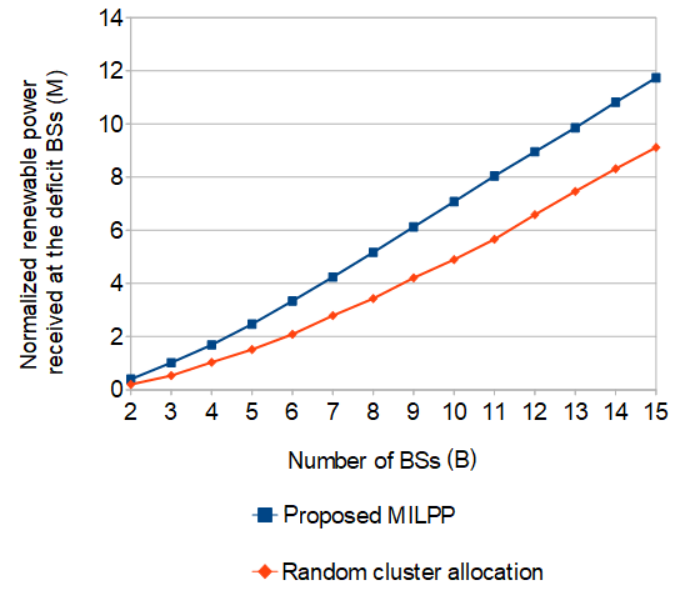
\includegraphics[width=0.75\columnwidth]{pictures/graph_1}
\caption{Average normalized renewable power received at the deficit BSs $M$ of the proposed MILPP and of random BS cluster allocation vs. number of BSs $B$. \label{graph_1}}
\end{figure}





Figure \ref{graph_2} shows the performance of the proposed MILPP and of random BS cluster allocation for different distribution line existence probabilities $q$. 
The performance gap between the two BS cluster allocations increases with the distribution line existence probability in the range of $0$ to $0.3$, whereas it is nearly constant in the range of $0.3$ to $1$. 

\begin{figure}[H]
\centering
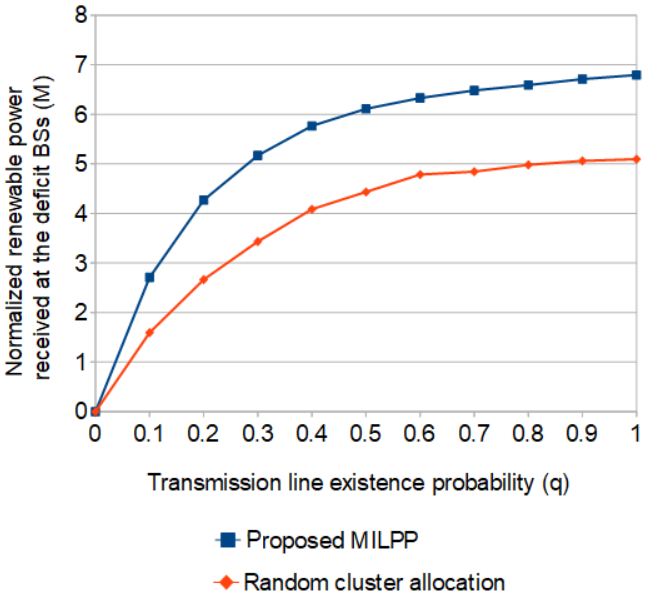
\includegraphics[width=0.75\columnwidth]{pictures/graph_2}
\caption{Average normalized renewable power received at the deficit BSs $M$ of the proposed MILPP and of random BS cluster allocation vs. distribution line existence probability $q$.\label{graph_2}}
\end{figure}






Figure \ref{graph_3} shows the performance of the proposed MILPP and of random BS cluster allocation for different power loss coefficients per $l$ meters of distribution line $C$\footnote{The normalized Euclidean distance $d\big((i,j)\big)=\frac{||BS_i - BS_j||}{l}$ is used in all formulas, derived parameters and  the proposed MILPP. Hence, the results in Figure \ref{graph_3} do not change with different values of $l$, only the scale of the x-axis changes. If the BSs  are deployed in an area of, e.g., 1000 m x 1000 m, Figure \ref{graph_3} should be read with the x-axis label “Power loss coefficient per 1000 meters.”}. 
The performance gap between the two BS cluster allocations decreases slightly with the power loss coefficient per $l$ meters of distribution line. 


\begin{figure}[H]
\centering
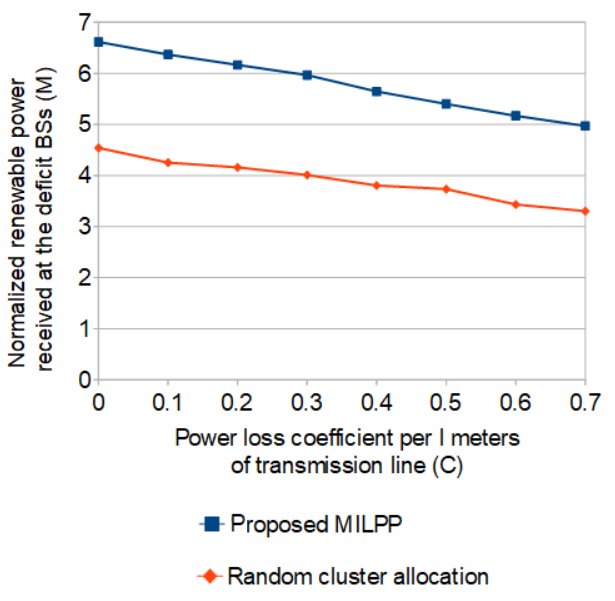
\includegraphics[width=0.75\columnwidth]{pictures/graph_3}
\caption{Average normalized renewable power received at the deficit BSs $M$ of the proposed MILPP and of random BS cluster allocation vs. power loss coefficient per $l$ meters of distribution line $C$.\label{graph_3}}
\end{figure}





Figure \ref{graph_4} shows the performance of the proposed MILPP and of random BS cluster allocation for different power surplus values $b_0$. $b_1$ was fixed to $-1$.
The performance gap between the two BS cluster allocations increases with the power surplus value in the range of $0$ to $1$, whereas it decreases in the range of $1$ to $2$. This is because the power was normalized with respect to $\max\{b_0,|b_1|\}$. If $b_0\neq 1$, either $\hat{b}_0$ or $|\hat{b}_1|$ is smaller than $1$ because a mismatch exists between the power surplus value  
and the power deficit value. Only if $b_0= 1$, $\hat{b}_0$ and $|\hat{b}_1|$ are both 1 because the power surplus value and the power deficit value have the same absolute value. 

\begin{figure}[H]
\centering
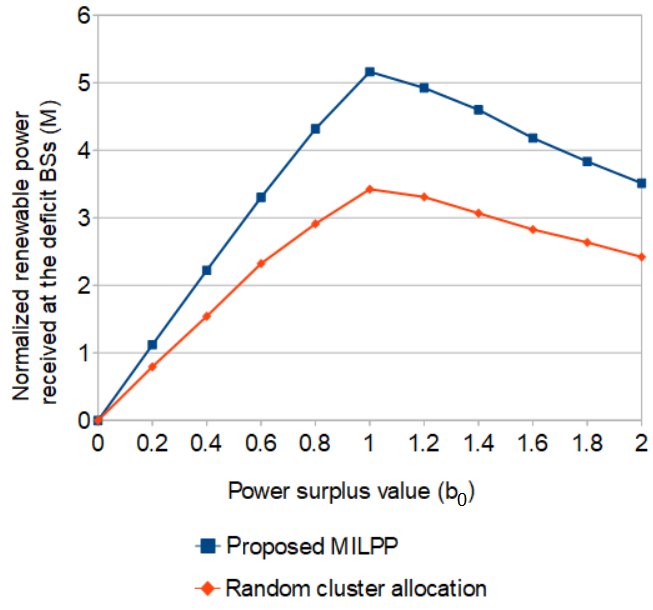
\includegraphics[width=0.75\columnwidth]{pictures/graph_5}
\caption[Average normalized renewable power received at the deficit BSs $M$ of the proposed MILPP and of random BS cluster allocation vs. power surplus value $b_0$]{Average normalized renewable power received at the deficit BSs $M$ of the proposed MILPP and of random BS cluster allocation vs. power surplus value $b_0$. $b_1$ was fixed \mbox{to $-1$.}\label{graph_4}}
\end{figure}

Figures \ref{graph_1} - \ref{graph_4} show that the proposed MILPP always outperforms the random BS cluster allocation because the MILPP considers the
topology of the cellular network and the power losses in the distribution lines. Because the proposed MILPP takes into account the topology of the cellular network,
it increases the probability that a BS is deployed with an energy harvester type that is anti-correlated to those deployed at its connected neighboring BSs. In addition, the shorter the distribution line between a pair of BSs, the more likely that these two BSs are deployed with anti-correlated energy harvesters, because the proposed MILPP takes into account the distance-dependent power loss in the distribution lines. The MILPP has an average system performance improvement of around $40\%$ in comparison with the random BS cluster allocation.





\section{Summary of Chapter \ref{Chapter_3}\label{sum_Chapter_3}}
In Chapter \ref{Chapter_3}, the system model was extended to a multi-cell cellular network. The system model consisted of several BSs that were distributed in an area and some of them were connected by distribution lines to share the renewable energy among them. There were two different types of energy harvesters, which have anti-correlated energy generation profiles, available for deployment in the system model. Two PV cells that have significantly different orientation angles, such as east-oriented and west-oriented PV cells, are an example for energy harvesters with anti-correlated energy generation profiles.
A mixed-integer linear programming problem (MILPP) was developed to determine what type of energy harvester should be deployed to every BS to share the renewable power most efficiently in the cellular network. The MILPP can be run once during the cellular network planning and it maximizes the power that can be transmitted from surplus BSs to deficit BSs in the cellular network.
The algorithm takes into account the topology of the cellular network, i.e., whether or not a distribution line exists between a pair of
BSs. Hence, the proposed algorithm increases the probability that a BS is deployed with an energy harvester type that is anti-correlated to those deployed at its connected neighboring BSs. In addition, the shorter the distribution line between a pair of BSs, the more likely that these two BSs are deployed with anti-correlated energy harvesters, because the proposed algorithm takes into account the distance-dependent power loss in the distribution lines. 
The renewable power that can be transmitted from the surplus BSs to the deficit BSs in the cellular network is on average around 40\% higher with the proposed MILPP in comparison with randomly deploying anti-correlated energy harvesters to the BSs.



